\documentclass[UTF8, xcolor=table]{beamer}
\usepackage{fontspec}
\setsansfont{宋体}
\usepackage{latexsym,amssymb,amsmath,amsbsy,amsopn,amstext,xcolor,multicol}
\usepackage{graphicx,wrapfig,fancybox}
\usepackage{pgf,pgfarrows,pgfnodes,pgfautomata,pgfheaps,pgfshade}
\usepackage{beamerthemeTsinghua}
\usepackage[backend=bibtex,style=numeric]{biblatex}
\usepackage{array}
\usepackage{bm}
\usepackage{caption}
\usepackage[caption=false]{subfig}
\usepackage{multirow}
\usepackage{booktabs}

\defbibheading{bibliography}[\bibname]{} %avoid printbibliography 自动生成目录
\addbibresource{resource/reference-utf8.bib}
%\setbeamertemplate{bibliography item}{\insertbiblabel} %将默认的丑陋的icon 改成数字,或者下面这个也行
\setbeamertemplate{bibliography item}[text] % [ref](http://tex.stackexchange.com/questions/68080/beamer-bibliography-icon)

\begin{document}

\setbeamerfont{footnote}{size=\tiny}
\setbeamerfont{caption}{size=\scriptsize}
\setbeamertemplate{caption}[numbered]


\title{Parallel construction for model-adaptive convex bounding polyhedron}
\author{TANG Lei, SHI Kanle, YONG Junhai. etc}
\institute{CG\&CAD, School of Software, Tsinghua University}
\date{2014-01-22}
%\date{\today}

\frame{
\titlepage
\vspace{-6mm}
\begin{figure}[htpb]
  \begin{center}
	
\includegraphics[width=0.2\linewidth]{Tsinghua_University_Logo.eps}
  \end{center}
\end{figure}
}

  \section*{目录}
  \frame {
    \frametitle{\secname}
    \tableofcontents
  }

  \AtBeginSubsection[] {
  \frame<handout:0> {
  \frametitle{目录}
  \tableofcontents[current,currentsubsection]
    }
  }

  \section{引言}

  %\subsection{背景}

  \frame{
  \frametitle{\subsecname~ 引言}
    包围体在计算机图形学和计算几何领域中应用广泛, 常用于加速几何求交、光线跟踪和碰撞检测等多种算法.

    \begin{figure}
    \centering
    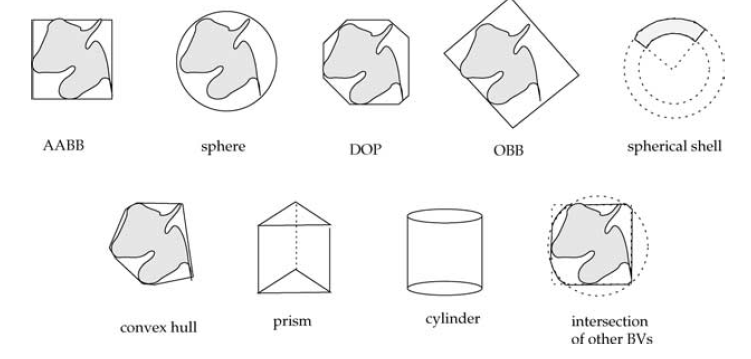
\includegraphics[width=2.5in]{resource/Teschner2005-bounding-volumes}
    \caption{各种各样的包围体\cite{teschner2005collision}}
    \label{Teschner2005-bounding-volumes}
    \end{figure}
    %常用的有: AABB, OBB, Sphere, $k$-Dop, 凸包, 以及 包围椭球、包围柱、Tribox和Zonotopese等.
  }

      \frame{
   \frametitle{\subsecname~ 引言}
   综合来看: \begin{description}
   \item[$k$-DOP\cite{klosowski1998efficient}]方向固定且有限, 不同模型其截面方向一致, 不够紧致.
   \item[凸包]很(最)紧致, 但面片数量太多, 复杂度$O(n\log n)$.
    \end{description}
   本文目标:\begin{description}
   \item[紧致]能够自适应模型
   \item[快速]利用GPU加速
   \item[灵活]通过参数~$k$~调节简单性和紧致性
    \end{description}
  }

  \section{模型适应的凸包围多面体构造算法}

    \subsection{问题定义及算法流程}

     \frame{
       \frametitle{问题的定义}
        由~$k$~个截面构成的凸包围多面体称为凸包围~$k$~面体($k$-Convex Bounding Polytope, 简称~$k$-CBP), 可通过~$k$~个半空间定义:
        \begin{equation}
        \label{equ:kcbp_definition}
        \left\{
        \begin{array}{l}
            k\mbox{-CBP} = \mathop  \bigcap \limits_{i = 1}^k \bm{H_i} \\
            \bm{H_i} = \left\{ {\left. {\bm{p} \in {\mathbb{R}^3}} \right| \bm{n_i} \cdot \bm{p} \le {w_i}} , w_i \in \mathbb{R} \right\},
        \end{array}
        \right.
        \end{equation}
        其中, $\bm{n_i}$~是半空间~$\bm{H_i}$~的法向, 方向指向包围体外部, $w_i$~是输入点集中沿~$\bm{n_i}$~方向投影的最大值.
    }

       \frame{
       \frametitle{算法流程}

        %\begin{figure}
        %\centering
        %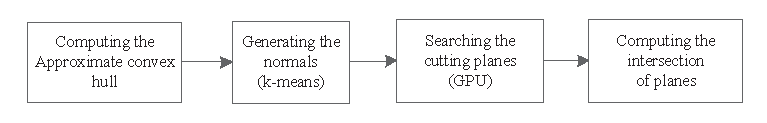
\includegraphics[width=4.0in]{resource/N112014-00019-2.eps}
        %\caption{算法流程图}
        %\label{lbl:kcbp-algorithm-flowchart}
        %\end{figure}

        \begin{description}
           \item[法向]结合近似内凸包和~$k$-means~
           \item[截面]GPU~中沿各法向搜索切点构造截面
           \item[交点]截面对偶映射求得交点
        \end{description}
    }

  \subsection{截面法向的生成}

    \frame{
        \frametitle{近似凸包的构造}
        \begin{figure}
        \vspace{-3mm}
        \subfloat[]
        {
           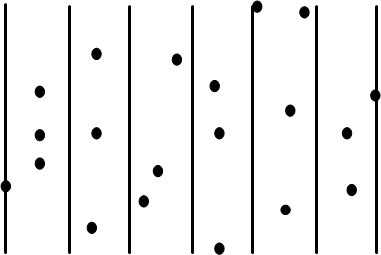
\includegraphics[width=0.28\textwidth]{resource/approximate-convexhull-step1.png}
        }\hspace{2mm}
        \subfloat[]
        {
            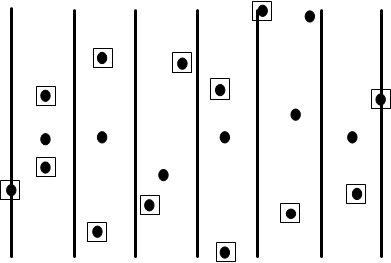
\includegraphics[width=0.28\textwidth]{resource/approximate-convexhull-step2.png}
        }\hspace{2mm}
        \subfloat[]
        {
           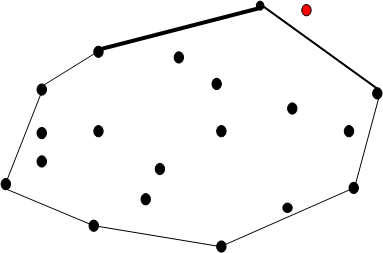
\includegraphics[width=0.28\textwidth]{resource/approximate-convexhull-step3.png}
        }
        \caption{二维近似内凸包的构造}
        \label{lbl:ach-2d}
        \end{figure}
        \vspace{-4mm}
        构造近似内凸包\cite{bentley1982approximation}, 算法复杂度为~$O(n+\xi)$, 扩展到三维为~$O(n+\xi^2\log\xi)$, 然后利用 $k$-means 聚类.
    }
    \frame{
        \frametitle{$k$-means 聚类}

        \begin{figure}
        \vspace{-5mm}
        \subfloat[]
        {
           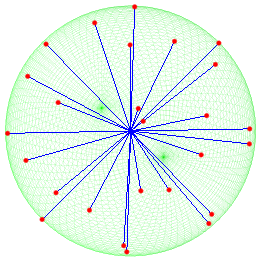
\includegraphics[width=0.28\textwidth]{resource/kmeans-init-normals-26.png}
        }
        \subfloat[]
        {
            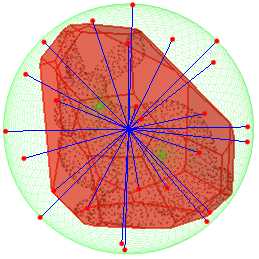
\includegraphics[width=0.28\textwidth]{resource/kmeans-init-normals-26-for-bunny.png}
        }
        \subfloat[]
        {
           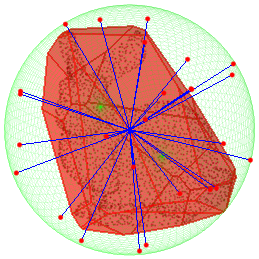
\includegraphics[width=0.28\textwidth]{resource/kmeans-cluster-normals-26-for-bunny.png}
        }
        \vspace{-2mm}
        \caption{通过聚类确定法向}
        \label{lbl:gen-fixed-normals}
        \end{figure}

        \vspace{-6mm}
        \small
        聚类初始方向(均匀分布). 距离度量(余弦), 聚类更新中心点时将面片的面积作为权重即$\bm{c_i}=\frac{\sum_{i=1}^{i=n} \omega_i \cdot \bm{n_i} } {\sum_{i=1}^{i=n} \omega_i}$, 其中$\bm{c_i}$ 为第~$i$~类的中心点, $\omega_i$~ 为法向~$\bm{n_i}$~所在面片对应的面积.
    }

  \subsection{搜索截面及求交}

    \frame{
    \frametitle{搜索截面}
     \footnotesize 等效于寻找最大投影值, 即对每个法向~$\bm{n_i}$, 从输入模型的所有点中寻找最大投影值的点作为切点进而确定~$\bm{n_i}$~对应的截面.
时间复杂度为~$O(k\cdot n)$, 其中~$k$~为法向数量, $n$~为模型所含点数. 各法向的计算相互独立, 借助~GPU~并行加速.

    \begin{figure}
    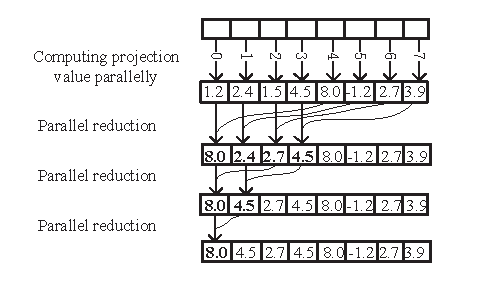
\includegraphics[width=2.5in]{resource/N112014-00019-6.eps}
    \caption{并行规约求最大投影值}
    \label{lbl:reduction-getmax}
    \end{figure}
    }

        \frame{
    \frametitle{求交算法}
      \small 法向~$\bm{n}(a,b,c)$~及平面上一点~$\bm{p}(x_0,y_0,z_0)$~确定, 转化为平面方程~$ax + by + cz = ax_0 + by_0 + cz_0=d$, $d \neq 0$. 对偶映射后的点为~$\bm{p'}(a/d, b/d, c/d)$, 对这~$k$~个映射点求凸包, 凸包平面映射回原来的交点, 时间复杂度为$O(k\log k$).

      亦可直接通过枚举所有每~3~个平面交于~1~点的情况, 然后排除在平面外部的交点, 剩下的构成~$k$-CBP~的顶点, 时间复杂度为$O(k^3$)\cite{ericson2005real}.
    }


  \section{实验与分析}

  \subsection{凸包围多面体的生成速度}

    \frame{
        \begin{figure}
         \vspace{-5mm}
        \subfloat%[Budda(31232 points)]
        {  \label{fig:exp:cpu:budda}
           \includegraphics[width=0.38\textwidth,page=2]{resource/N112014-00019-7.pdf}
        }
        \subfloat%[Dinosaur(40277 points)]
        {  \label{fig:exp:cpu:Dinasour}
            \includegraphics[width=0.38\textwidth, page=3]{resource/N112014-00019-7.pdf}
        }\linebreak %强制换行
        \vspace{-5mm}%
       \subfloat%[Alice(224291 points)]
        {  \label{fig:exp:cpu:alice}
           \includegraphics[width=0.38\textwidth, page=4]{resource/N112014-00019-7.pdf}
        }
        \subfloat%[Bugatti(1010815 points)]
        {  \label{fig:exp:cpu:buggatti}
           \includegraphics[width=0.38\textwidth, page=5]{resource/N112014-00019-7.pdf}
        }
        \caption{本文算法与~CPU~算法对比\tiny Budda(31k),Dinosaur(40k),Alice(224k), Bugatti(1011k)}
        \label{chart:exps:cputime}
        \end{figure}
    }

    \frame{
        图~\ref{chart:exps:cputime} 中横纵坐标分别代表多面体面数和运行时间, 其中虚线代表搜索截面的过程, 实线为构造凸包围多面体总体耗时. 当模型点数量较大时, 搜索截面的过程占据了算法绝大多数时间, 且随着凸包围多面体的面数~$k$~ 值增加而线性增长, 这与搜索截面时间复杂度($O(k\cdot n)$)一致, 截面求交过程的时间复杂度为$O(k\log k)$,
当点数量极大时, 实线虚线几乎重合即求交等步骤耗时相比整体算法而言几乎可忽略.
    }

    \frame{
     \vspace{-7mm}
        \begin{table} \tiny
        \caption{本文算法与文献\cite{karlsson2010parallel}算法对比}
        %\centerline{\zihao{-5}\bf \small 表1\quad 本文算法与文献~${[21]}$~算法对比}
        %\centerline{\footnotesize{\bf Table 1}\quad Comparison of result between ${[21]}$ and ours}
        %\begin{center}\belowrulesep=0pt\renewcommand{\arraystretch}{1.3} \doublerulesep 0.4pt \tabcolsep 15pt
        \begin{tabular}{p{1.5cm}<{\centering}ccc ccc} %p本身占一列
        \hline
        \multirow{2}{*}{$k$} & \multicolumn{3}{c}{Apple(8118 points)} & \multicolumn{3}{c}{~~~~~Bugatti(1010815 points)}\\
        %\cmidrule(lr){2-4}\cmidrule(lr){5-7}
        %\hline
        %\rowcolor[gray]{0.9} $k$ &
        ~&SSE$^{5}(ms)$ & $k$-CBP(ms) &  Speedup &SSE(ms) & $k$-CBP(ms) &  Speedup \\
        \hline
        6 & 0.4 & 0.12  & 3.20     & 24.2 & 3.20  & 7.56 \\
        16 & 0.9 & 0.26  & 3.43    & 44.5 & 8.44  & 5.27 \\
        26 & 1.4 & 0.41  & 3.38    & 66.5 & 13.65  & 4.87 \\
        36 & 1.9 & 0.52  & 3.65    & 91.1 & 18.34  & 4.97 \\
        46 & 2.5 & 0.67  & 3.74    & 119.5 & 24.13  & 4.95 \\
        56 & 2.9 & 0.79  & 3.66    & 138.4 & 28.86  & 4.80 \\
        66 & 3.5 & 0.95  & 3.69    & 170.6 & 34.10  & 5.00 \\
        76 & 4.0 & 1.08  & 3.70      & 197.1 & 39.85  & 4.95 \\
        86 & 4.5 & 1.22  & 3.69    & 219.8 & 45.08  & 4.88 \\
        106 & 5.4 & 1.49  & 3.62   & 267.8 & 55.52  & 4.82 \\
        136 &  6.8 & 1.92  & 3.54  & 342.9 & 71.24  & 4.81 \\
        156 &  7.7 & 2.17  & 3.55  & 411.3 & 81.18  & 5.07 \\
        186 &  9.3 & 2.60  & 3.58  & 479.4 & 97.39  & 4.92 \\
        206 &  10.5 & 2.85  & 3.68 & 523.0 & 106.87  & 4.89  \\  \hline
        \end{tabular}
        \label{tab:exp:sse-time}
        \end{table}
        \vspace{-3mm}
    \scriptsize 点数量较小时, 能够提高~3-4~倍速度,模型变大, 加速比更大, ~Bugatti~模型的提速达到~4-8~倍.
    }

  \subsection{凸包围多面体的紧致程度}

   \frame{

        \begin{figure}
         \vspace{-5mm}
        \subfloat
        {  \label{fig:exp:cpu:budda}
           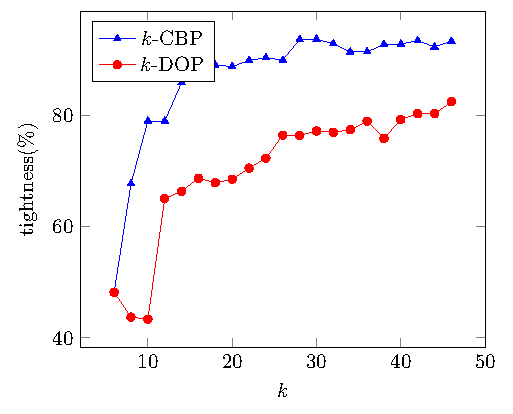
\includegraphics[width=0.35\textwidth,page=1]{resource/N112014-00019-8.pdf}
        }
        \subfloat
        {  \label{fig:exp:cpu:Dinasour}
            \includegraphics[width=0.35\textwidth, page=2]{resource/N112014-00019-8.pdf}
        }\linebreak %强制换行
        \vspace{-3mm}%
       \subfloat%[Alice(224291 points)]
        {  \label{fig:exp:cpu:alice}
           \includegraphics[width=0.35\textwidth, page=3]{resource/N112014-00019-8.pdf}
        }
        \subfloat%[Bugatti(1010815 points)]
        {  \label{fig:exp:cpu:buggatti}
           \includegraphics[width=0.35\textwidth, page=4]{resource/N112014-00019-8.pdf}
        }
        \caption{紧致程度对比: $k$-DOP v.s $k$-CBP \tiny Apple(8k), Budda(31k), Dinosaur(40k), Alice(224k)}
        \label{chart:exps:tightness}
        \end{figure}
        \vspace{-8mm}
        紧致程度用凸包与凸包围多面体的体积之比来量化.
    }


    \frame{


        \begin{table}
        \scriptsize
        \caption{\label{tab:exp:cgal}$k$-CBP~与~QuickHull~凸包算法比较}
         %\centerline{\zihao{-5}\bf \small 表2\quad $k$-CBP~与~QuickHull~凸包算法比较}
        %\centerline{\footnotesize{\bf Table 2}\quad Comparison of result between QuickHull and $k$-CBP}
        %\vspace{3mm}{\zihao{6}\footnotesize
        %\begin{center}\belowrulesep=0pt\renewcommand{\arraystretch}{1.3} \doublerulesep 0.4pt \tabcolsep 10pt
         \begin{tabular}{lcccccl}
          \toprule
          Model & f(CHull)& f($k$-CBP) & $\tau$ ($k$-CBP) & t(CHull(ms)) & t($k$-CBP(ms))\\ % 后面重新跑的, KCBP加上了近似凸包及求交时间的总和, 和近似凸包的分组时间也加了.
          \midrule
          Apple	& 499 & 30 & 93.67\% & 5.5 & 1.30\\ % apple3  自己电脑跑的数据, 之前是用的chengxianyu的电脑.
          Budda	& 1608 & 46 & 92.39\% & 21.3 & 2.86 \\ %  1.0+0.86+1
          Dinosaur	& 1240 & 44 & 93.34\% & 22.6 & 1.99 \\  % 1.0+0.98+0.1
          Alice	& 1332 & 44 & 93.92\% & 85.8 & 8.47\\ % 2+6.48
          Bugatti & 24654 & 44 & 95.06\% & 688.7 & 25.41\\
          \bottomrule
         \end{tabular}
         \vspace{-2mm}
        \end{table}

        \small  $\tau$($k$-CBP)~为凸包围多面体的紧致程度. 与凸包相比, 本文算法在大大简化包围体平面数量的同时能保持较好的紧致程度, 下图为可视化结果.
    }

    \frame{
%          \begin{figure}
%    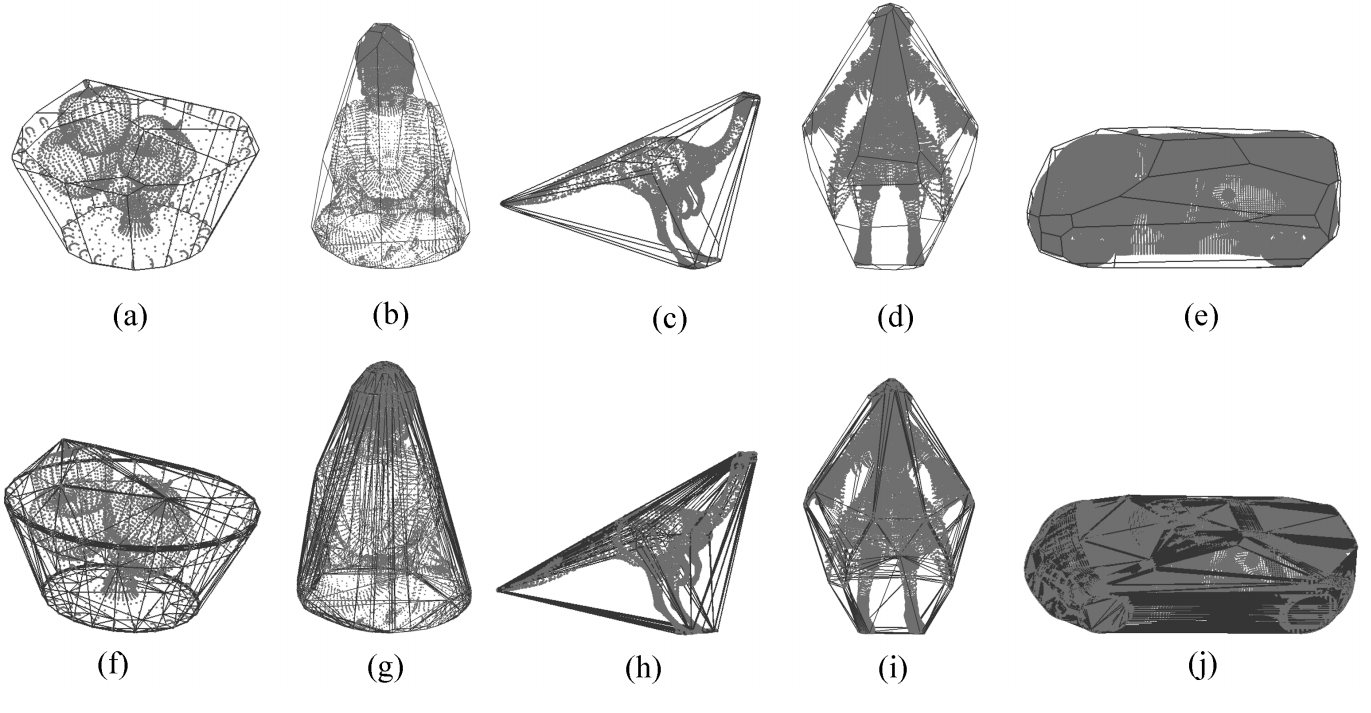
\includegraphics[width=4.0in]{resource/N112014-00019-9}
%    \caption{$k$-CBP~与凸包对比: \tiny (a) Apple (30-CBP); (b) Budda (46-CBP); (c) Dina-
%sour (44-CBP); (d) Alice (44-CBP); (e) Bugatti (44-CBP); (f) Apple (CHull); (g) Budda (CHull); (h) Dinosaur (CHull);
%(i) Alice (CHull); (j) Bugatti (CHull)}
%    \label{pic:exps:ch-kcbp}
%    \end{figure}

    \begin{figure}
    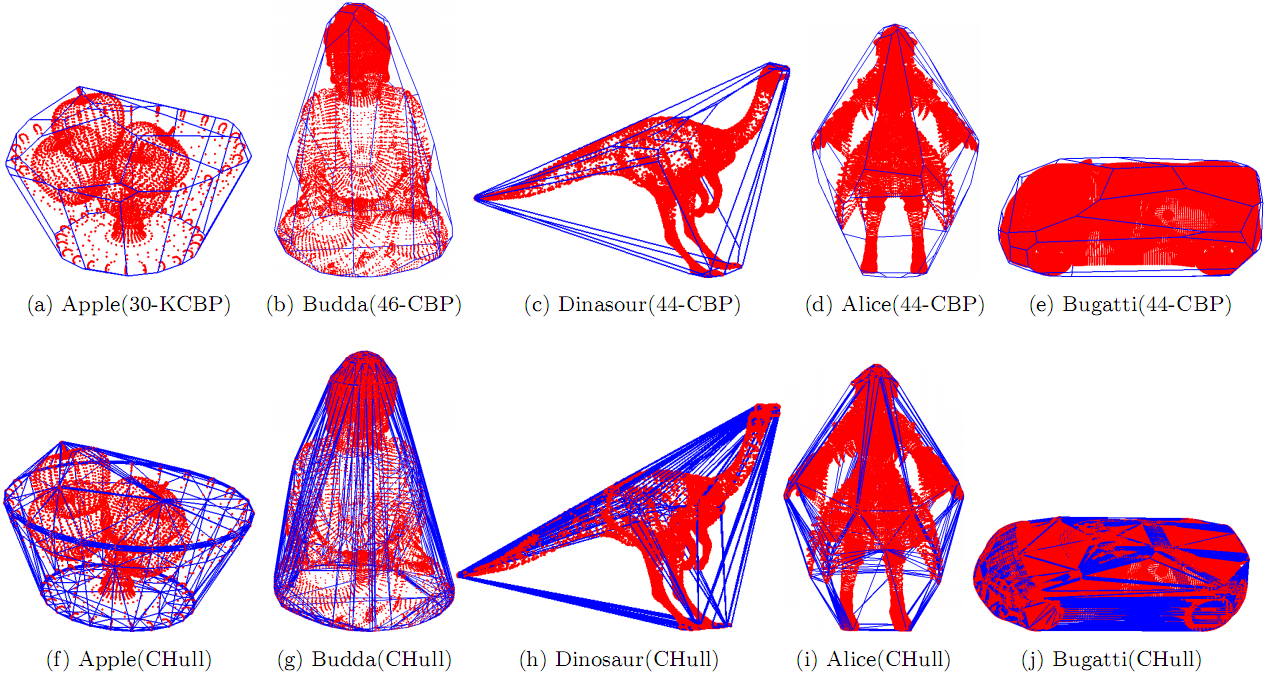
\includegraphics[width=4.0in]{resource/kcbp-convexhull.png}
    \caption{$k$-CBP~与凸包对比}
    \label{pic:exps:ch-kcbp}
    \end{figure}

    }

      \subsection{凸包围多面体的简单应用}

    \frame{
        \begin{figure}
        \centering
        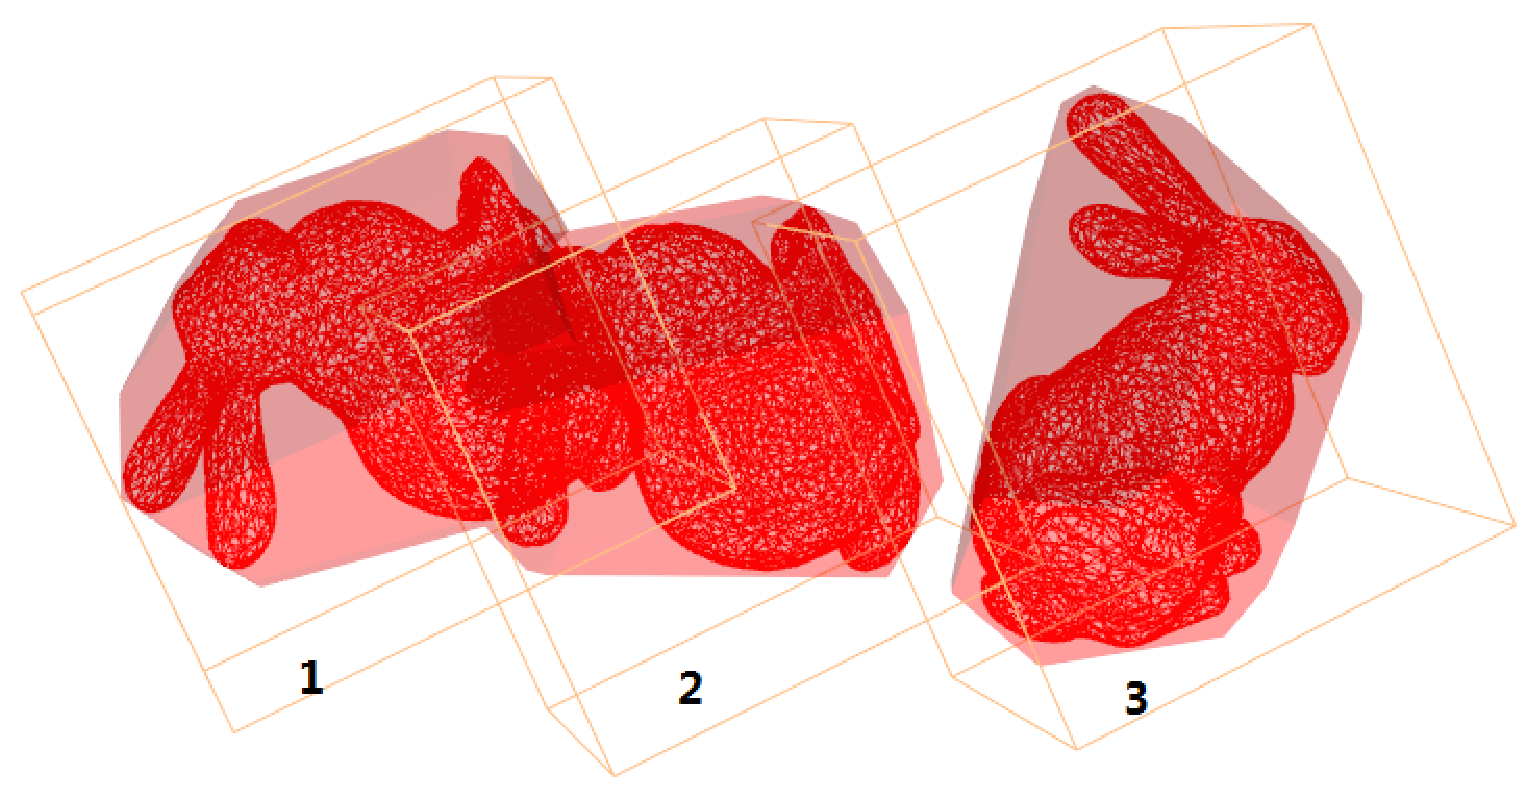
\includegraphics[width=3in]{resource/N112014-00019-10.eps}
        \caption{~$k-$CBP~应用于碰撞检测示例}
        %\centerline{\bahao\bf 图 10\quad ~$k-$CBP~应用于碰撞检测示例}
        %\centerline{\footnotesize {\bf Figure 10}\quad  Example of collision detection using $k$-CBP}
        \label{lbl:bunny-box-kcbp-collsion-detection-example}
        \end{figure}

        \small 图中模型~1~与~2、2~与~3~的包围盒分别相交, 而其~$16$-CBP~仅~1~与~2~相交, 实际模型仅~1~与~2~相交. 不同数量的模型(模型位置和旋转角度随机生成)测试结果如下表所示.
    }

    \frame{
        \begin{table}
        \tiny
        \centering
         \caption{\label{tab:exp:box:kcbp:collsiondetection}$k$-CBP~和包围盒应用于碰撞检测结果对比}
        % \centerline{\zihao{-5}\bf \small 表4\quad }
        %\centerline{\footnotesize{\bf Table 4}\quad Comparison of result of collision detection between $k$-CBP and bounding box}
        %\vspace{3mm}{\zihao{6}\footnotesize
        %\begin{center}\belowrulesep=0pt\renewcommand{\arraystretch}{1.3} \doublerulesep 0.4pt \tabcolsep 10pt
         \begin{tabular}{lccccccl}
          \toprule
          n& c(Box) & c($16$-CBP) &  t(Box) & t($16$-CBP) & r(Box) & r($k$-CBP) & n(Model) \\
          \midrule
           10 & 0.1 & 1.8 &    26.0  & 0.1    & 0.00 \% &  100.00\% & 0\\
           30 & 0.2 & 2.9 &   134.0  & 70.0   & 45.45\% & 83.33\% & 5\\
           50 & 0.5 & 4.8 &   506.0  & 255.2  & 46.34\% & 86.36\% & 19 \\
           70 & 0.4 & 4.8 &   901.1  & 492.5  & 44.16\% & 80.95\% & 34 \\
           90 & 0.7 & 5.7 &  1324.0  & 734.7  & 41.82\% & 73.02\% & 46 \\
          100 & 0.7 & 7.8 &  1481.0  & 870.7  & 43.31\% & 75.34\% & 55 \\
          150 & 1.0 & 9.8 &  4153.1  & 2473.0 & 42.98\% & 70.75\% & 150 \\
          200 & 1.6 & 12.8 & 8049.3  & 4430.9 & 41.02\% & 71.32\% & 281 \\
          \bottomrule
         \end{tabular}
         % \end{center}}\vspace{-2mm}
        \end{table}
        \small 其中~r(Box), r($16$-CBP)分别表示包围盒、16-CBP~的命中率即用实际模型相交的数量除以包围体检测出来相交的数量. 模型和凸包围多面体是否相交都采用了普通~AABB~ 树的方式进行判断.
    }

    \section{主要参考文献}
    \frame[t,allowframebreaks]{
      \frametitle{\secname}
    \scriptsize
    \printbibliography
    }

    \section{FAQ}
    \frame{
      \frametitle{\secname}
       Thank you!
    }
    
    


\end{document}

